\section{Evaluation}
\label{sec:eval}

\subsection{Experimental Settings}
\begin{figure}[h]
  \centering
  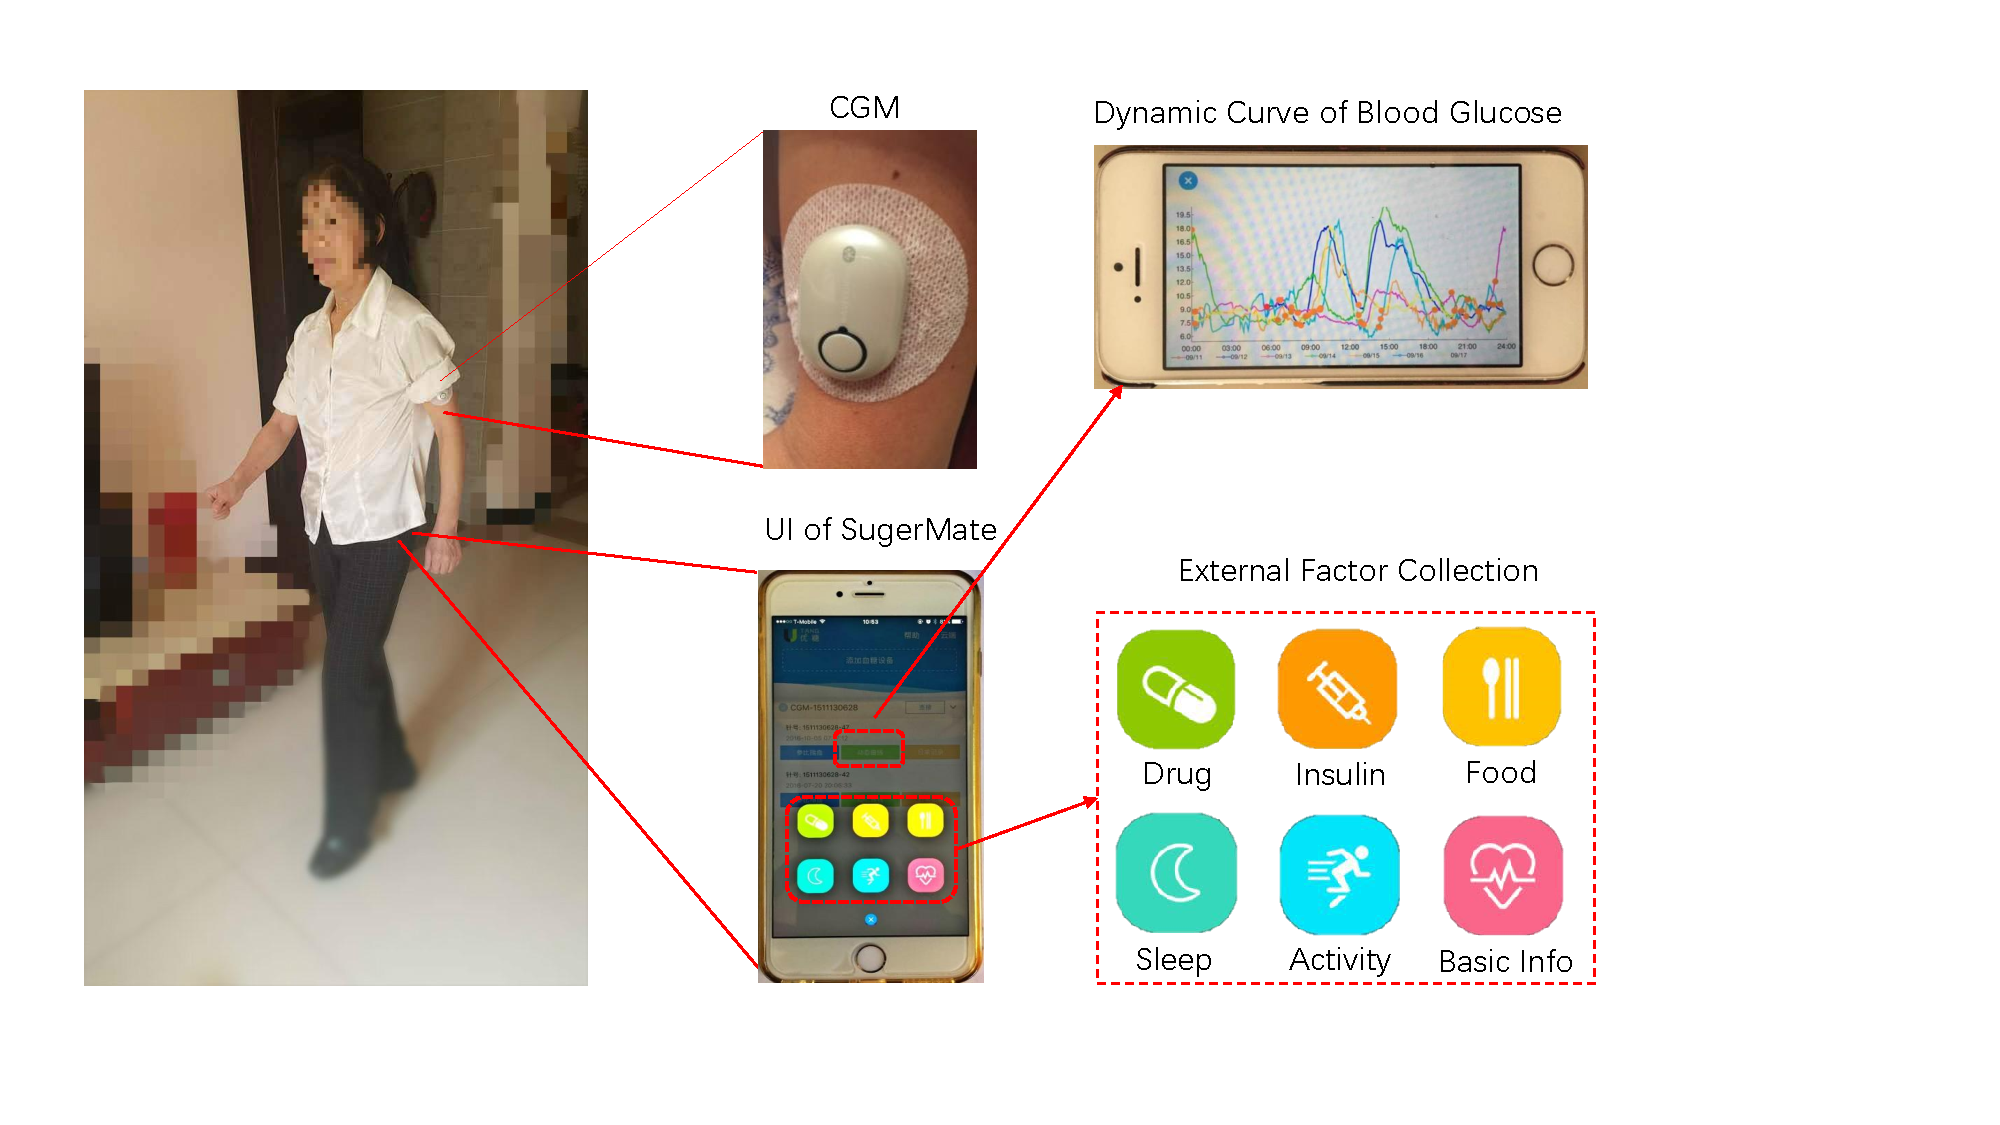
\includegraphics[width=0.7\columnwidth]{./img/UI1.pdf}
  \caption{An illustration of the equipments for data collection. Each participant wears a CGM device to record blood glucose concentration and uses a smartphone to collect external factors. }
  \label{fig:experiment_case}
\end{figure}
\begin{figure}[h]
  \centering
  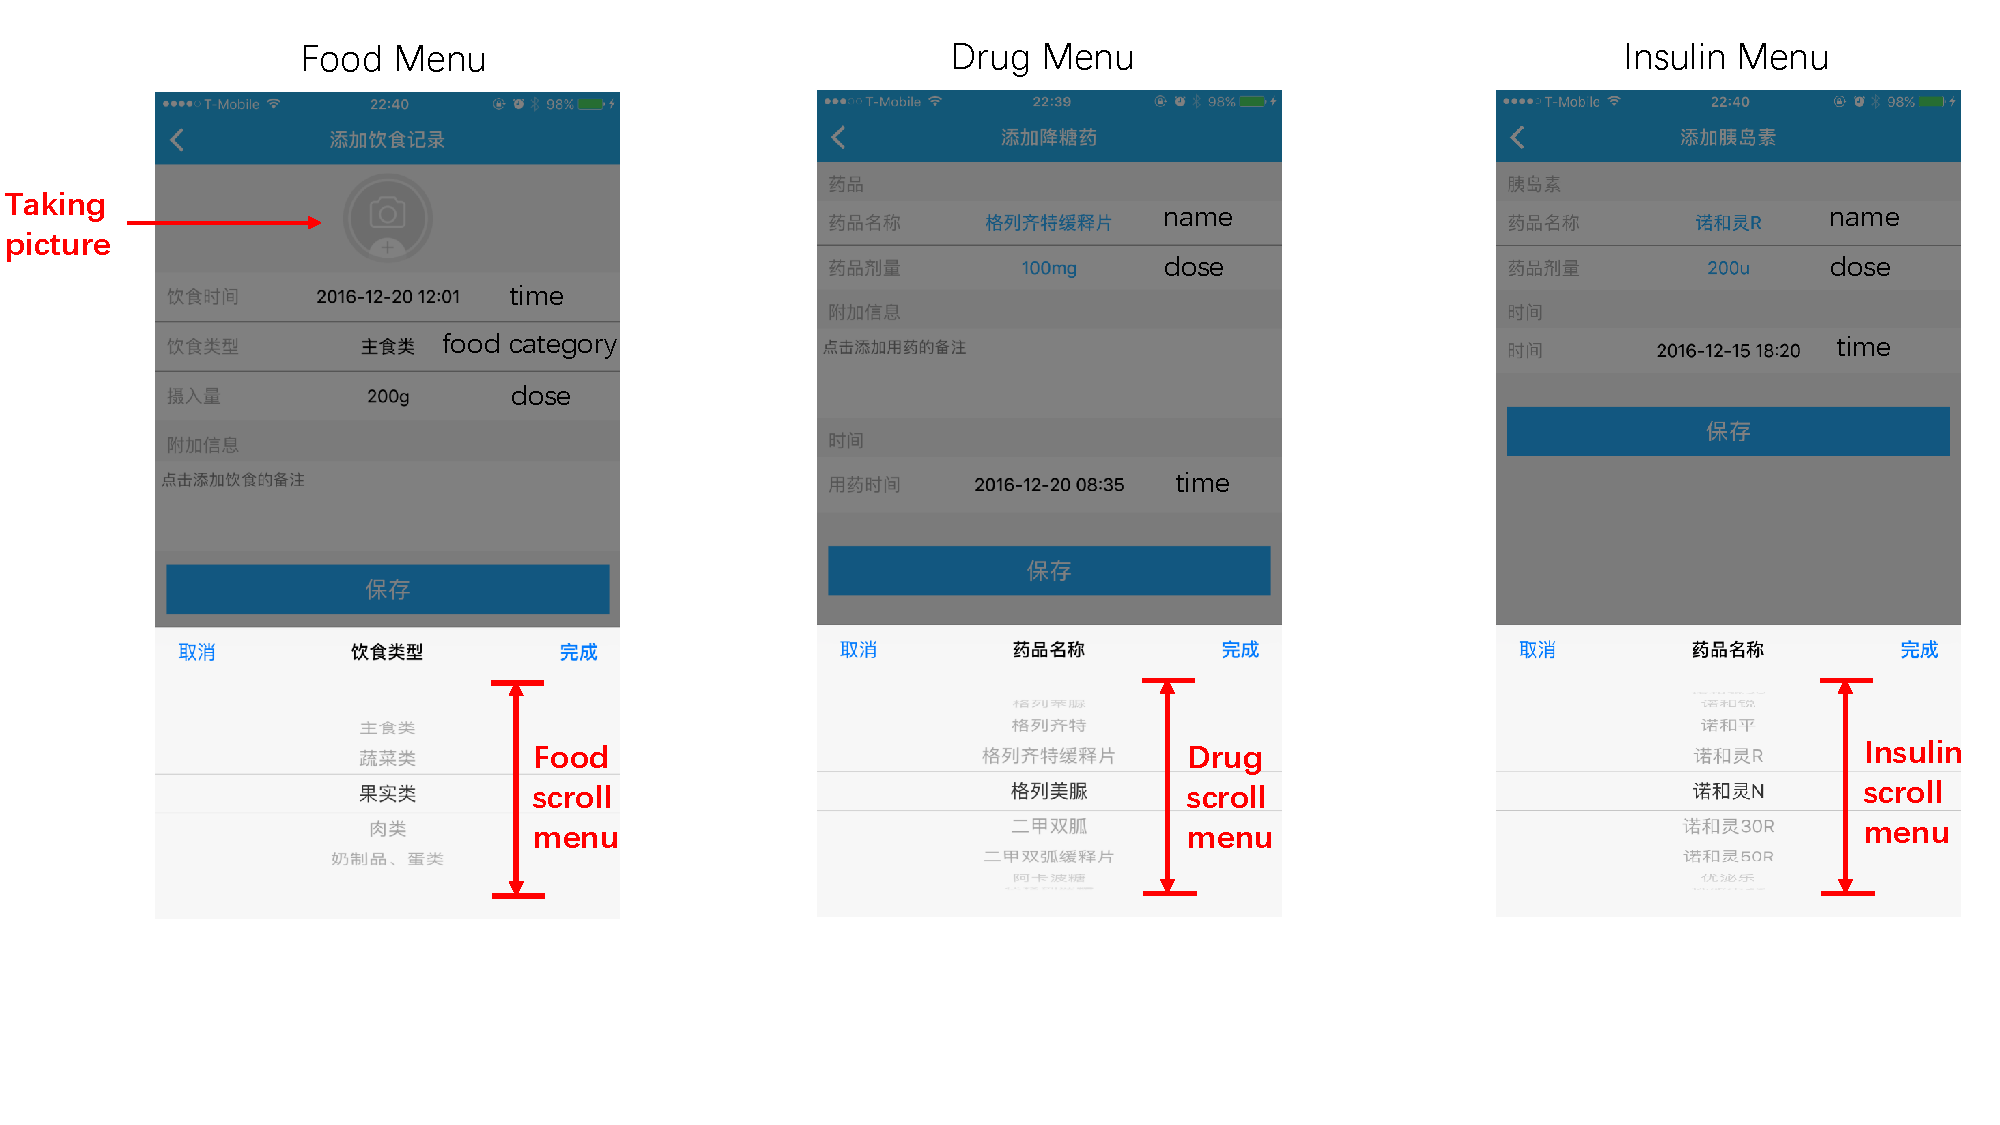
\includegraphics[width=0.9\columnwidth]{./img/usibility_UI.pdf}
  \caption{\rev{User interfaces for food, drug and insulin intake recording.}}
  \label{fig:usibility_UI}
\end{figure}


\textbf{Datasets.}
We validate \sysname on a dataset of $112$ participants ($35$ non-diabetes, $38$ type I diabetic patients and $39$ type II diabetic patients) collected from July 2016 to January 2017.
Each participant is equipped with (1) a WAVEGUIDER \emph{U-Tang} CGM device~\cite{bib:CGM_wave} to record blood glucose concentration every $3$ minutes and (2) a smartphone with \sysname installed to collect external factors either automatically (activities and sleep quality) or manually (food, drug, and insulin intake).
All participants agree to take measurements (\ie wear the CGM device and use \sysname to record external factors) for at least $6$ days, which is a normal disposable usage duration of the enzyme in the sensor of the CGM.
\figref{fig:experiment_case} illustrates an example of data collection from a user.
\rev{\figref{fig:usibility_UI} shows the user interfaces for manual recording of food, drug and insulin intake.}
In total we obtain 762639 samples of blood glucose concentration and the corresponding external factors covering around 38132 hours.
In brief, we collect the following categories of data:
\begin{itemize}
  \item
  \textbf{Meta information.}
  We record basic personal data including gender, age, weight and health status to cover a wide range of users.
  \tabref{tab:parcitipant} summarizes the basic information of the participants.
  \item
  \textbf{Blood glucose measurements.}
  We collect blood glucose measurements using commercial CGM devices for 6 to 30 days as labeled data.
  \tabref{tab:bgdata} summarizes the blood glucose measurements in our evaluation.
  \item
  \textbf{External factor measurements.}
  During measurements of blood glucose concentration, each participant manually inputs the times of their daily meal, drug and insulin intake.
  \sysname automatically records activity levels and sleep quality as in \secref{subsec:external}.
  \figref{fig:experiment_case} shows the user interfaces to record external factors.
\end{itemize}

\begin{table}
  \centering
  \caption{Summary of participant information.}
  \label{tab:parcitipant}
  \subfloat[]{%
  \begin{tabular}{cc}
  \toprule
  \textbf{Age (year)} & \textbf{\# User} \\
  \midrule
  15-24 & 8 \\
  25-34 & 17 \\
  35-44 & 24 \\
  45-54 & 29 \\
  55-64 & 34 \\
  \bottomrule
  \end{tabular}}%
  \quad% --- set horizontal distance between tables here
  \subfloat[]{%
  \begin{tabular}{ccc}
  \toprule
  \textbf{Weight} &\textbf{BMI ($kg/m^2$)}\cite{bib:world2013bmi} &\textbf{\# User} \\
  \midrule
  Underweight & (0,  18.5) & 18 \\
  Normal weight & [18.5,  25) & 31 \\
  Overweight &  [25,  30) &41 \\
  Obese &  [30, +$\infty$) & 22 \\
  \bottomrule
  \end{tabular}}%
  \quad%
%  \%subfloat[]{%
%  \begin{tabular}{cc}
%  \toprule
%  \textbf{Status} & \textbf{\# User} \\
%  \midrule
%  Non-diabetes & 35 \\
%  Type I & 38 \\
%  Type II & 39 \\
%  \bottomrule
%  \end{tabular}}
%  \quad%
  \subfloat[]{%
  \begin{tabular}{cc}
  \toprule
  \textbf{Gender} & \textbf{\# User} \\
  \midrule
  Male & 57 \\
  Female & 55\\
  \bottomrule
  \end{tabular}}
\end{table}

\begin{table}
  \centering
  \caption{Summary of blood glucose measurements.}
  \label{tab:bgdata}
  \subfloat[]{%
  \begin{tabular}{cc}
  \toprule
  \textbf{Duration (days)} & \textbf{\# User} \\
  \midrule
  6-10 & 48 \\
  11-15 & 24 \\
  16-20 & 20 \\
  21-25 & 13 \\
  26-30 & 7 \\
  \bottomrule
  \end{tabular}}%
  \qquad% --- set horizontal distance between tables here
  \subfloat[]{%
  \begin{tabular}{cc}
  \toprule
  \textbf{Blood Glucose} & \textbf{\# Sample} \\
  \midrule
  Level 1 & 75369 \\
  Level 2 & 293530 \\
  Level 3 & 235686 \\
  Level 4 & 158054 \\
  Total & 762639 \\
  \bottomrule
  \end{tabular}}%
\end{table}

\textbf{Ground Truth.}
We use the blood glucose concentrations collected by the CGM device as ground truth \footnote{While clinical studies report that the precision and accuracy of commercial CGM devices still need improving~\cite{bib:MEP08:Do, bib:JDST10:Vaddiraju}, they are sufficient as ground truth for the four normal and abnormal blood glucose levels.}. Note that the ground truth is required for the purpose of system evaluation.
\rev{In real world deployment, users are only required to wear the CGM in a calibration period for labeled examples, but do not need to wear CGM for the whole process of the blood glucose measurement.}

\textbf{Metrics.}
We mainly adopt precision, recall and accuracy~\cite{prf1} to quantify the performance of \sysname.

\subsection{Inference Accuracy}
\subsubsection{Overall Inference Accuracy}
Since all participants collected both measurements of CGM and external factors for at least 6 days, we use measurements during the former 5 days for training and the rest for testing.
\tabref{tab:confusion_matrix} shows the overall performance of \sysname.
All results are averaged over the testing data.
As shown, the recalls and the precisions for all the 4 blood glucose levels are above 79\% and 73\%, respectively.
In particular, the recalls for Level 1 (low blood glucose) and Level 4 (high blood glucose) are 83.13\% and 85.23\%, even though the training data for Level 1 and Level 4 only take up around 10\% and 20\% of the entire training set.
This result shows that \sysname can accurately infer low/high blood levels even with an imbalanced training dataset.
Overall, \sysname yields an accuracy of 82.14\%, shows a promising performance to track blood glucose levels.
\rev{As a supplement of the professional blood glucose measurements, it is a screening tool for users to acknowledge their blood glucose while users cannot measure blood glucose by CGM or finger sticker.
Moreover, since \sysname holds the high recall in Level 1 and Level 4 detection, it is sensitive to detect the abnormal cases.
When SugarMate detects the abnormal cases, it will ask the users to have a double-check by CGM or finger stickers and take corresponding treatment.}

\begin{table}[h]
  \centering
  \caption{Confusion matrix of \sysname.}
  \label{tab:confusion_matrix}
  \begin{tabular}{|c|c|c|c|c|l|l|}
  \hline
  \multirow{2}{*}{\textbf{\begin{tabular}[c]{@{}c@{}}Ground\\ Truth\end{tabular}}} & \multicolumn{4}{c|}{\textbf{Inference}}                                                                                 & \multicolumn{2}{l|}{\multirow{2}{*}{}}\\
  \cline{2-5} & Level 1 & Level 2 & Level 3 & Level 4 & \multicolumn{2}{l|}{}
  \\ \hline
  Level 1 & \cellcolor[gray]{0.8}62657 & 5521 & 3672 & 3519 & 83.13\% & \multirow{4}{*}{\rotatebox{90}{\textbf{Recall}} } \\
  \cline{1-6}
  Level 2 & 16346 &  \cellcolor[gray]{0.8}240584 & 27563 & 9037 & 81.96\% & \\
  \cline{1-6}
  Level 3 & 2660 & 30905 & \cellcolor[gray]{0.8}188472 & 13649 & 79.97\% & \\
  \cline{1-6}
  Level 4 & 3443 & 5620 & 14278 & \cellcolor[gray]{0.8}134713 & 85.23\% & \\
  \hline
  \multicolumn{1}{|l|}{\multirow{2}{*}{}} & \multicolumn{1}{l|}{73.62\%} & \multicolumn{1}{l|}{85.12\%} & \multicolumn{1}{l|}{80.55\%} & \multicolumn{1}{l|}{83.72\%} & \multicolumn{2}{l|}{\multirow{2}{*}{\begin{tabular}[c]{@{}l@{}}Accuracy:\\ 82.14\%\end{tabular}}} \\
  \cline{2-5}
  \multicolumn{1}{|l|}{} & \multicolumn{4}{c|}{\textbf{Precision}} & \multicolumn{2}{l|}{} \\
  \hline
\end{tabular}
\end{table}


\subsubsection{Inference Result Analysis}
\label{subsec:predict_result_analysis}
To understand the inference accuracy and the risks of different types of errors in the context of blood glucose management, we classify the inference results based on the principles of Clarke Error Grid Analysis (CEGA) \cite{bib:DTT05:Clarke}.
The analysis classifies the inference results into correct event (Type A) and different types of errors (Type B to Type E) with increasing levels of severity.
For instance, Type B errors are those that will not lead to inappropriate treatments, while Type E errors can lead to wrong treatment.
\tabref{predict_results} summarizes the percentages of each type of results.
As shown, \sysname will not cause inappropriate treatment (Type A and B) in almost 90\% of the cases.
It may lead to unnecessary worries or treatment (Type C) in 5.47\% of the cases.
In fewer than 5\% of the cases, \sysname will miss an abnormal blood glucose event (Type D) or confuse treatment (Type E).
Therefore, \sysname is suitable as an temporal alternative for CGM devices.
However, we do not recommend \sysname for extended duration of usage for patients serious diabetics, who need regular blood glucose management.

\begin{table}[h]
  \centering
  \small
  \caption{Clarke error grid analysis}
  \label{predict_results}
  \begin{tabular}{|c|l|c|}
  \hline
  \textbf{Type of Result} & \multicolumn{1}{c|}{\textbf{Explanation of Result}} & \textbf{Percentage} \\
  \hline
  Type A & \begin{tabular}[c]{@{}l@{}}The inference value is consistent with the true value.\\ (\ie the inference blood glucose level is correct.)\end{tabular}                                                                                             & 82.14\% \\ \hline
  Type B & \begin{tabular}[c]{@{}l@{}}The inference result would not lead to inappropriate treatment. \\ (\ie Level 2 is predicted as Level 3, or vice-versa.)\end{tabular} & 7.67\% \\ \hline
  Type C & \begin{tabular}[c]{@{}l@{}}The inference result will lead to unnecessary treatment. \\ (\emph{i.e.}, Level 2 is predicted as Level 1/4,or Level 3 is predicted as Level 1/4.)\end{tabular} & 5.47\% \\ \hline
  Type D & \begin{tabular}[c]{@{}l@{}}Fail to detect hypoglycemia or hyperglycemia.\\ (\ie Level 1/4 are predicted as Level 2/3.)\end{tabular} & 3.81\% \\ \hline
  Type E & \begin{tabular}[c]{@{}l@{}}The predicted results that would confuse treatment by mistaking hypoglycemia\\ for hyperglycemia or vice-versa.\\ (\ie Level 1 is predicted as Level 4, and vice-versa.)\end{tabular} & 0.91\% \\ \hline
\end{tabular}
\end{table}


\subsubsection{Temporal View of Inference Results}
\label{subsec:Inference_Results}
\figref{fig:pre_gt} plots the inference results of \sysname of three participants (one non-diabetic, one Type I diabetic patient, and one Type II diabetic patient) throughout a day.
The errors are depicted at the bottom of each figure.
As shown, the true blood glucose levels vary during the day after important daily activities such as food intake (5:50, 11:20 and 19:00 for the non-diabetic user; 6:00 and 16:50 for the Type I diabetic user; 6:00, 12:50 and 17:45 for the Type II user), insulin injection (7:40 for the Type I diabetic user), drug intake (15:10 for the Type II user) and exercises (15:30 for the Type II user), indicating the importance of external factors.
The blood glucose levels inferred by \sysname match the true blood glucose levels most of the time.
\rev{Most errors mistake level 2 and level 3, and the errors often occur during the transition of two levels (\eg from 6:10 to 6:30 for the Type II diabetic user), or in case of sudden change of blood glucose concentration (\eg at 2:30 for the non-diabetic user and at 0:30 for the Type I diabetic user).
Nevertheless, these errors belong to the Type B errors in \secref{subsec:predict_result_analysis}, which will not lead to inappropriate treatment.}

\begin{table}[h]
  \centering
  \small
  \caption{\rev{Summary of average false positives and false negative per user.}}
  \label{tab:fpfn}
  \begin{tabular}{|l|c|c|c|c|c|c|}
  \hline
  \textbf{Level} & \multicolumn{1}{l|}{\textbf{FP (Day)}} & \multicolumn{1}{l|}{\textbf{FP (Hour)}} & \multicolumn{1}{l|}{\textbf{FPR}} & \multicolumn{1}{l|}{\textbf{FN (Day)}} & \multicolumn{1}{l|}{\textbf{FN (Hour)}} & \multicolumn{1}{l|}{\textbf{FNR}}
  \\ \hline
  Level 1 & 14.12 & 0.59 & 2.94\% & 8.00 & 0.33 & 1.67\% \\ \hline
  Level 2 & 26.46 & 1.10 & 5.51\% & 33.32 & 1.39 & 6.94\% \\ \hline
  Level 3 & 28.64 & 1.19 & 5.97\% & 29.71 & 1.24 & 6.19\% \\ \hline
  Level 4 & 16.49 & 0.69 & 3.44\% & 14.69 & 0.61 & 3.06\% \\ \hline
\end{tabular}
\end{table}


\rev{Table~\ref{tab:fpfn} shows the average false positives (FP) and false negatives (FN) per day and per hour for each user.
Given an inference every 3 minutes or 480 inferences per day, the number of FPs and FNs per hour is no greater than two.
Since only FPs for Level 1 and 4 will cause annoying notifications, such situations occur at an even lower rate.
To further reduce the unnecessary notifications, \sysname only reminds the user when there are three consecutive inferences of Level 1 or Level 4.
This mechanism is acceptable because (a) most errors occur during transition of blood glucose levels or when there is a sudden change of blood glucose concentration and (b) the 9-minute delay usually will still save sufficient time for proper treatment \cite{bib:Low_Blood_Glucose_(Hypoglycemia)} \cite{bib:whitmer2009hypoglycemic}.
}

\begin{figure}[h]
  \centering
  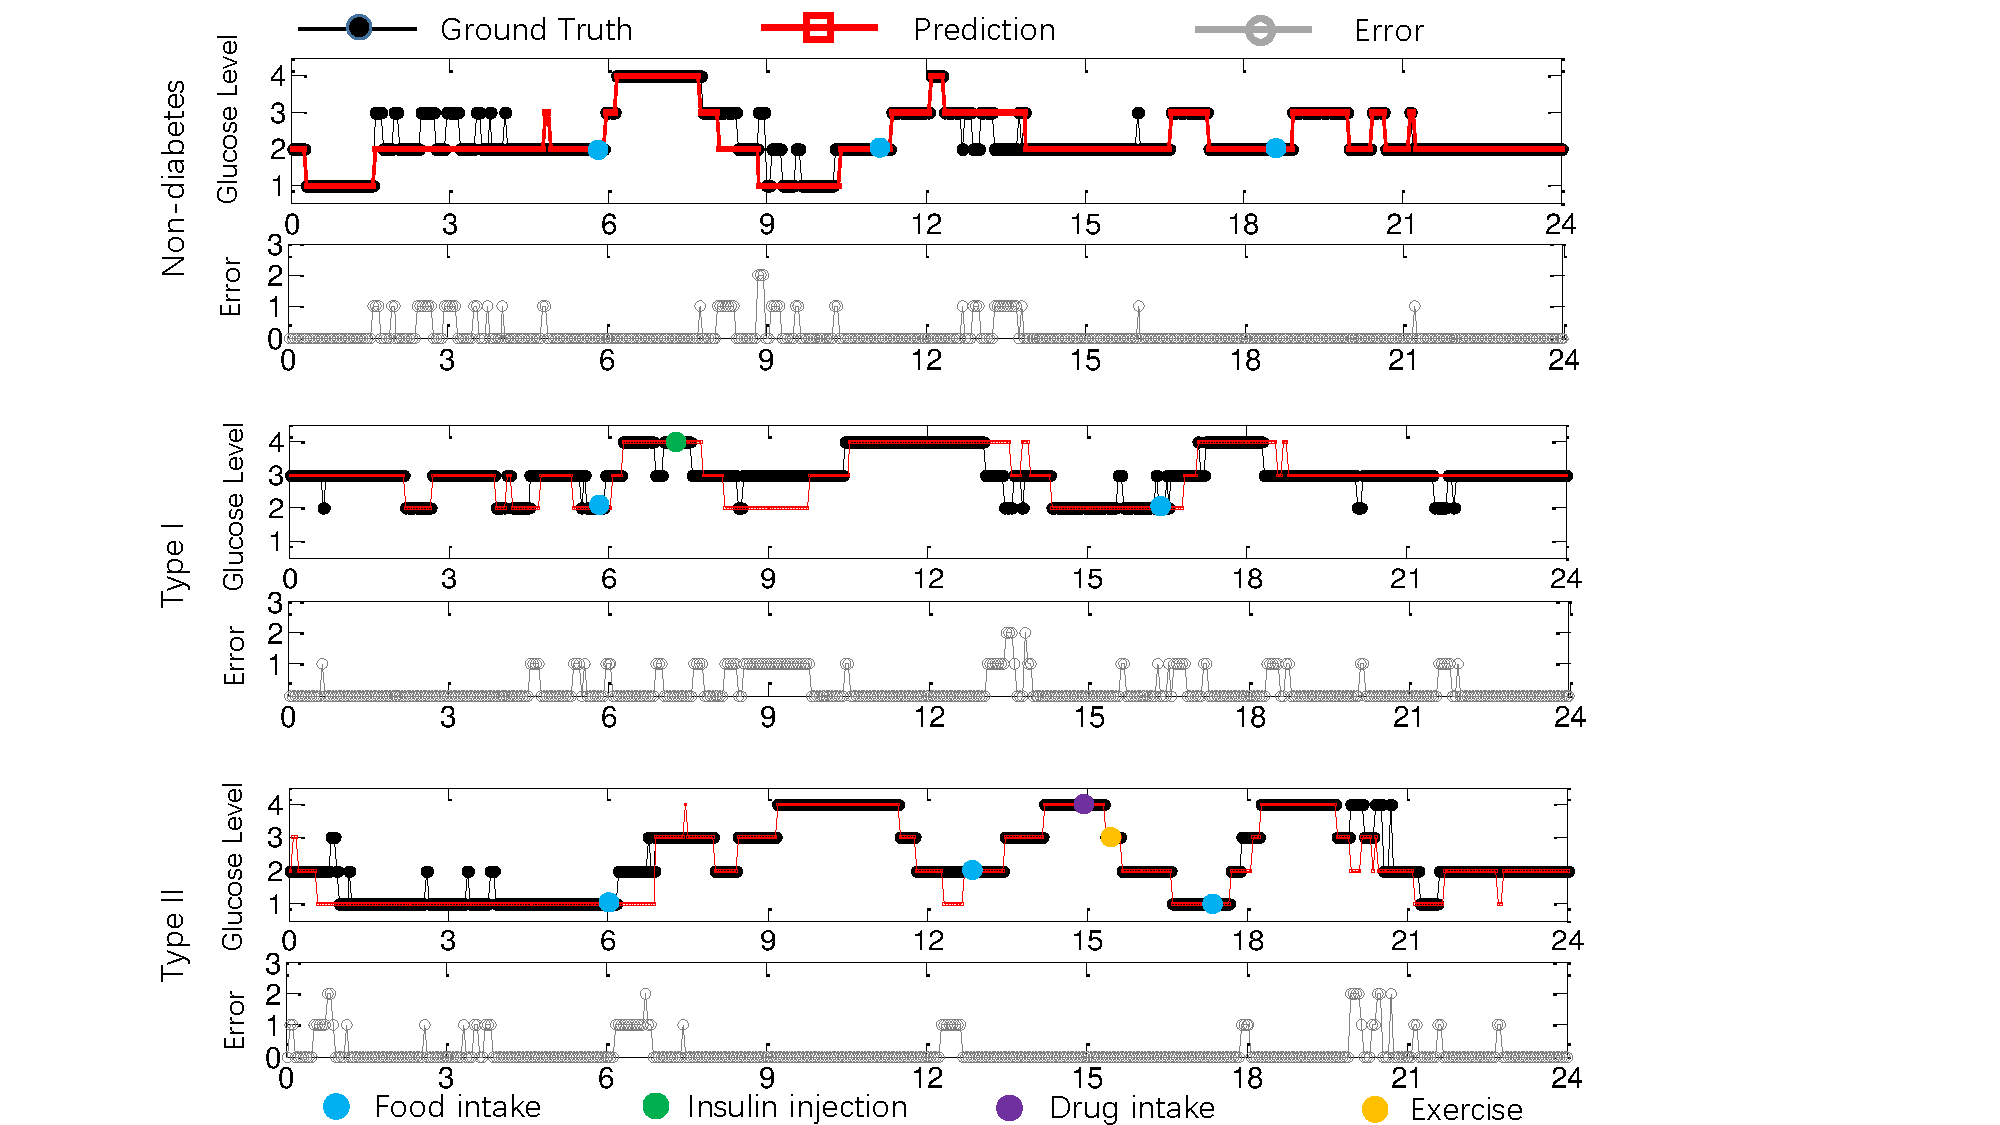
\includegraphics[width=0.8\columnwidth]{./img/pred_vs_gt2.pdf}
  \caption{Traces of blood glucose level inference results throughout a day.}
  \label{fig:pre_gt}
\end{figure}

\subsection{Model Comparison}

\subsubsection{Effectiveness of \modelname Framework}
\rev{To demonstrate the effectiveness of the multi-division framework in making full use of the dataset, we evaluate \modelname by 10-fold cross validation from two perspectives.}

\fakeparagraph{Layer contribution analysis}
To evaluate the effect of different layers, we conduct blood glucose level inference with three combinations of layers.
\begin{itemize}
  \item
  \emph{Deep dynamic layer.}
  Training without considering differences in groups and persons, and only output a general model.
  \item
  \emph{Deep dynamic layer + Grouped input layer.}
  Learn group-specific feature representations but ignore per-person characteristics in the output.
  \item
  \emph{Deep dynamic layer + Grouped input layer + personalized output layer (\modelname).}
  Efficiently learn features from different groups and output personalized inference results.
\end{itemize}
\figref{fig:cmp_model} plots the comparison results of the three combinations.
As shown, both the precisions and recalls increase with more layers, with an improvement of 21.13\% in average precision and 18.57\% in average recall, respectively.
Moreover, the standard deviations (error bars) drop remarkably from 17.25\% to 10.25\%  of average precision, and from 20.75\% to 10.75\% of average recall.
The results demonstrate the effectiveness of \modelname, which learns representative features from the same groups and considers individual differences in blood glucose level inference.

\begin{figure}[h]
  \centering
  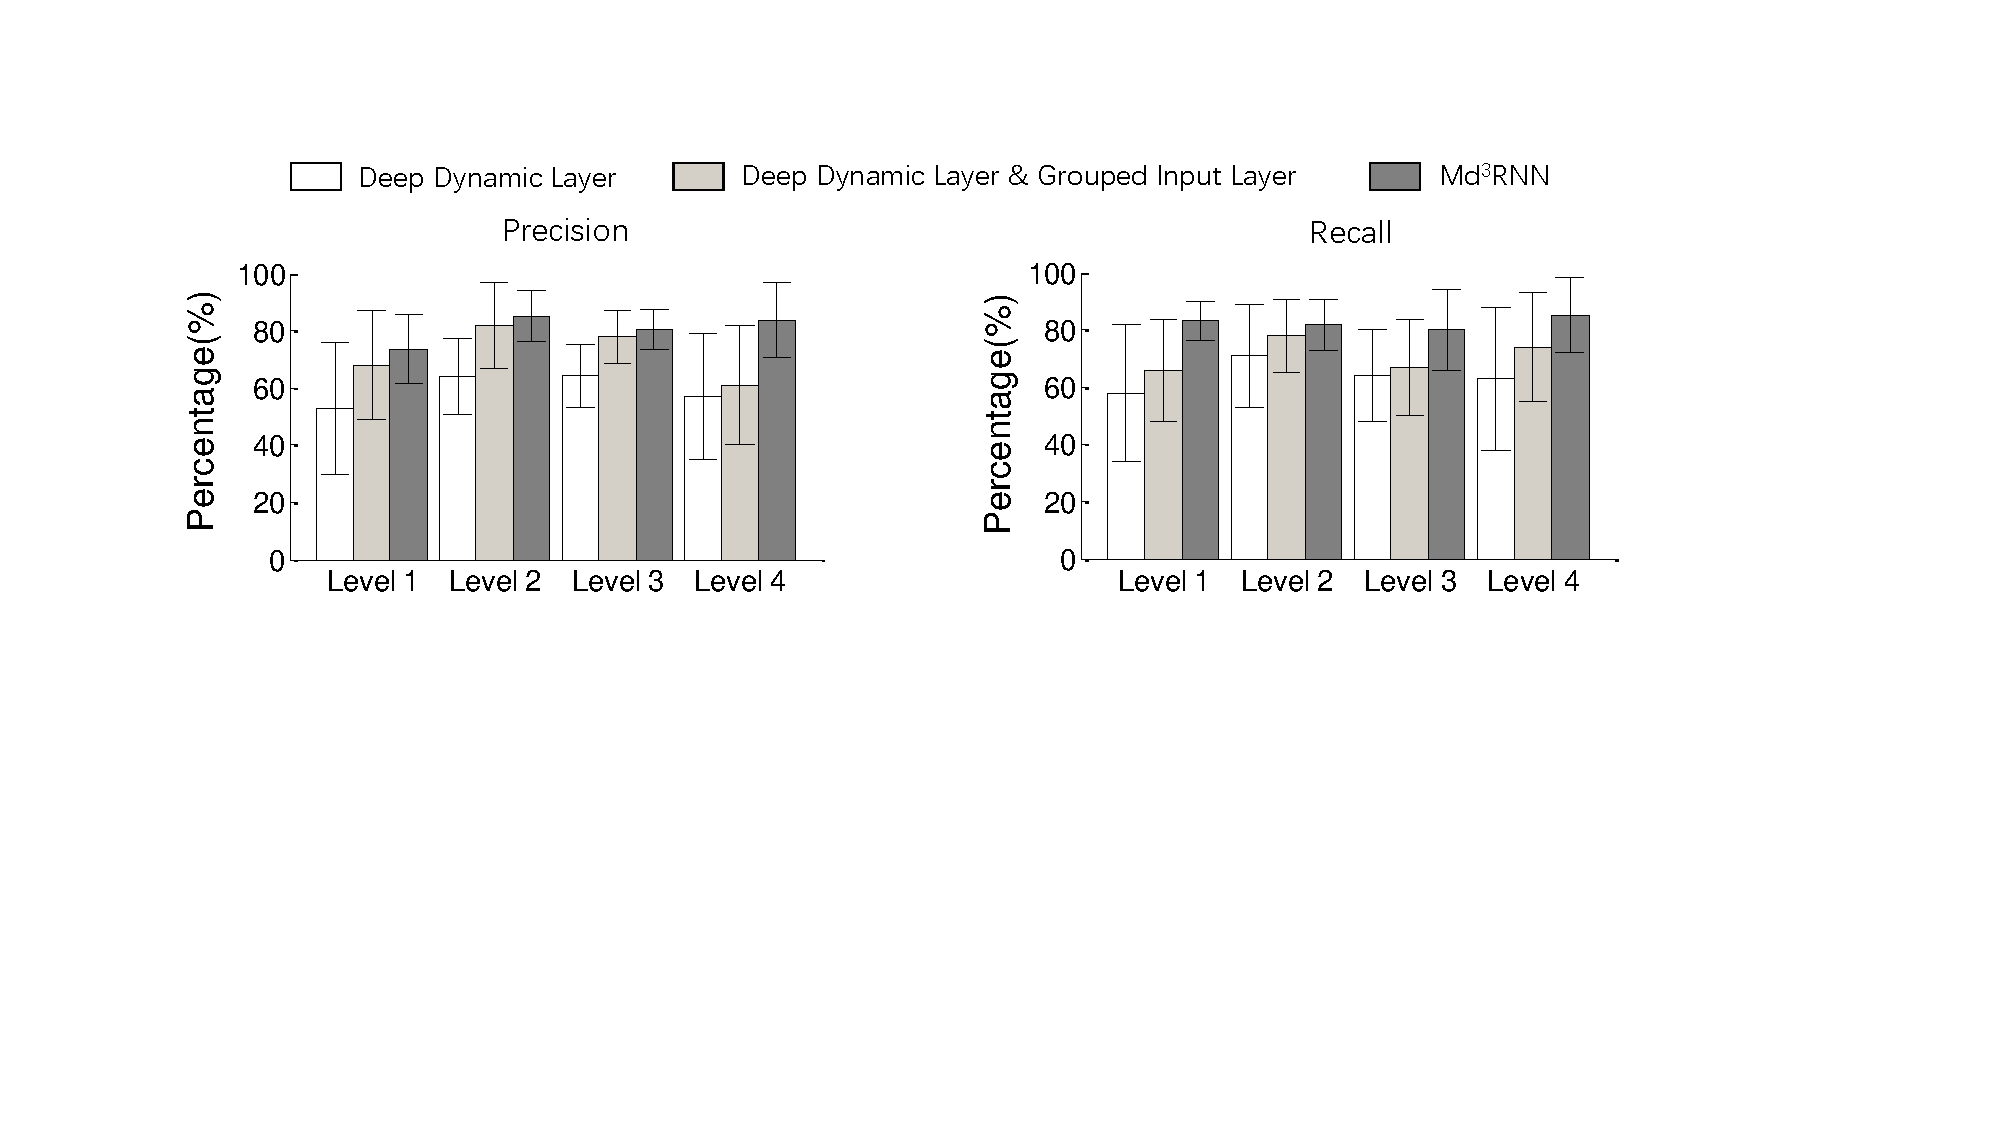
\includegraphics[width=0.8\columnwidth]{./img/CMP_Models2.pdf}
  \caption{Performance of layer combinations. \rev{The error bars denote the standard deviations on 10-fold cross-validation.}}
  \label{fig:cmp_model}
\end{figure}

\fakeparagraph{Comparison of data sharing schemes}
To demonstrate the benefits of sharing data and knowledge among groups and users, we compare \modelname with other learning frameworks with different data sharing schemes.
\begin{itemize}
  \item \emph{General Learning.}
  All the training data are directly fed into the model (\ie deep RNN) for training indifferently.
  General learning results in a \emph{generic} model that assumes universal correlations between all inputs and the blood glucose levels.
  \item \emph{Group Learning.}
  The data of users belonging to a same group are fed into a model (\ie deep RNN) for training.
  Three separate models are obtained for three groups (\ie non-diabetic, type I and type II diabetic).
  The group learning results in a \emph{group} model that shares the general characteristics of users within the same group but without data sharing among users in different groups.
  \item \emph{Single Learning.}
  We train a different model (\ie deep RNN) for each individual participant by feeding his/her own measurements into the model.
  Single learning results in a \emph{personalized} model without sharing data and learning knowledge from measurements of other participants.
\end{itemize}

\figref{fig:cmp_multi_division} shows the overall precisions and recalls of our \modelname as well as \emph{General learning}, \emph{Group learning} and \emph{Single learning}.
As shown, our multi-divisional learning framework (\modelname) performs best among the four learning approaches with an average precision of 80.75\% and an average recall of 82.57\%.
It also yields the lowest standard deviations (17.18\% of average precision and 17\% of average recall).
The results show that \modelname is both effective and stable in blood glucose level inference.

General learning treats each sample of training data equally, and ignores the individual differences, so it performs poorly in most cases.
\rev{Conversely, single learning approach encodes the individual characteristics but suffers from lacking of user-specific training dataset. It may require a very large learning personalized data to achieve an effective result.} Even though group learning learns the similarities of users within the same group, it ignores inter-person physiological differences.
\modelname combines the advantages of these three learning approaches, which makes better use of the limited individual training data by sharing measurements among users and preserves user-specific characteristics via the personal learning layer.

\begin{figure}[h]
  \centering
  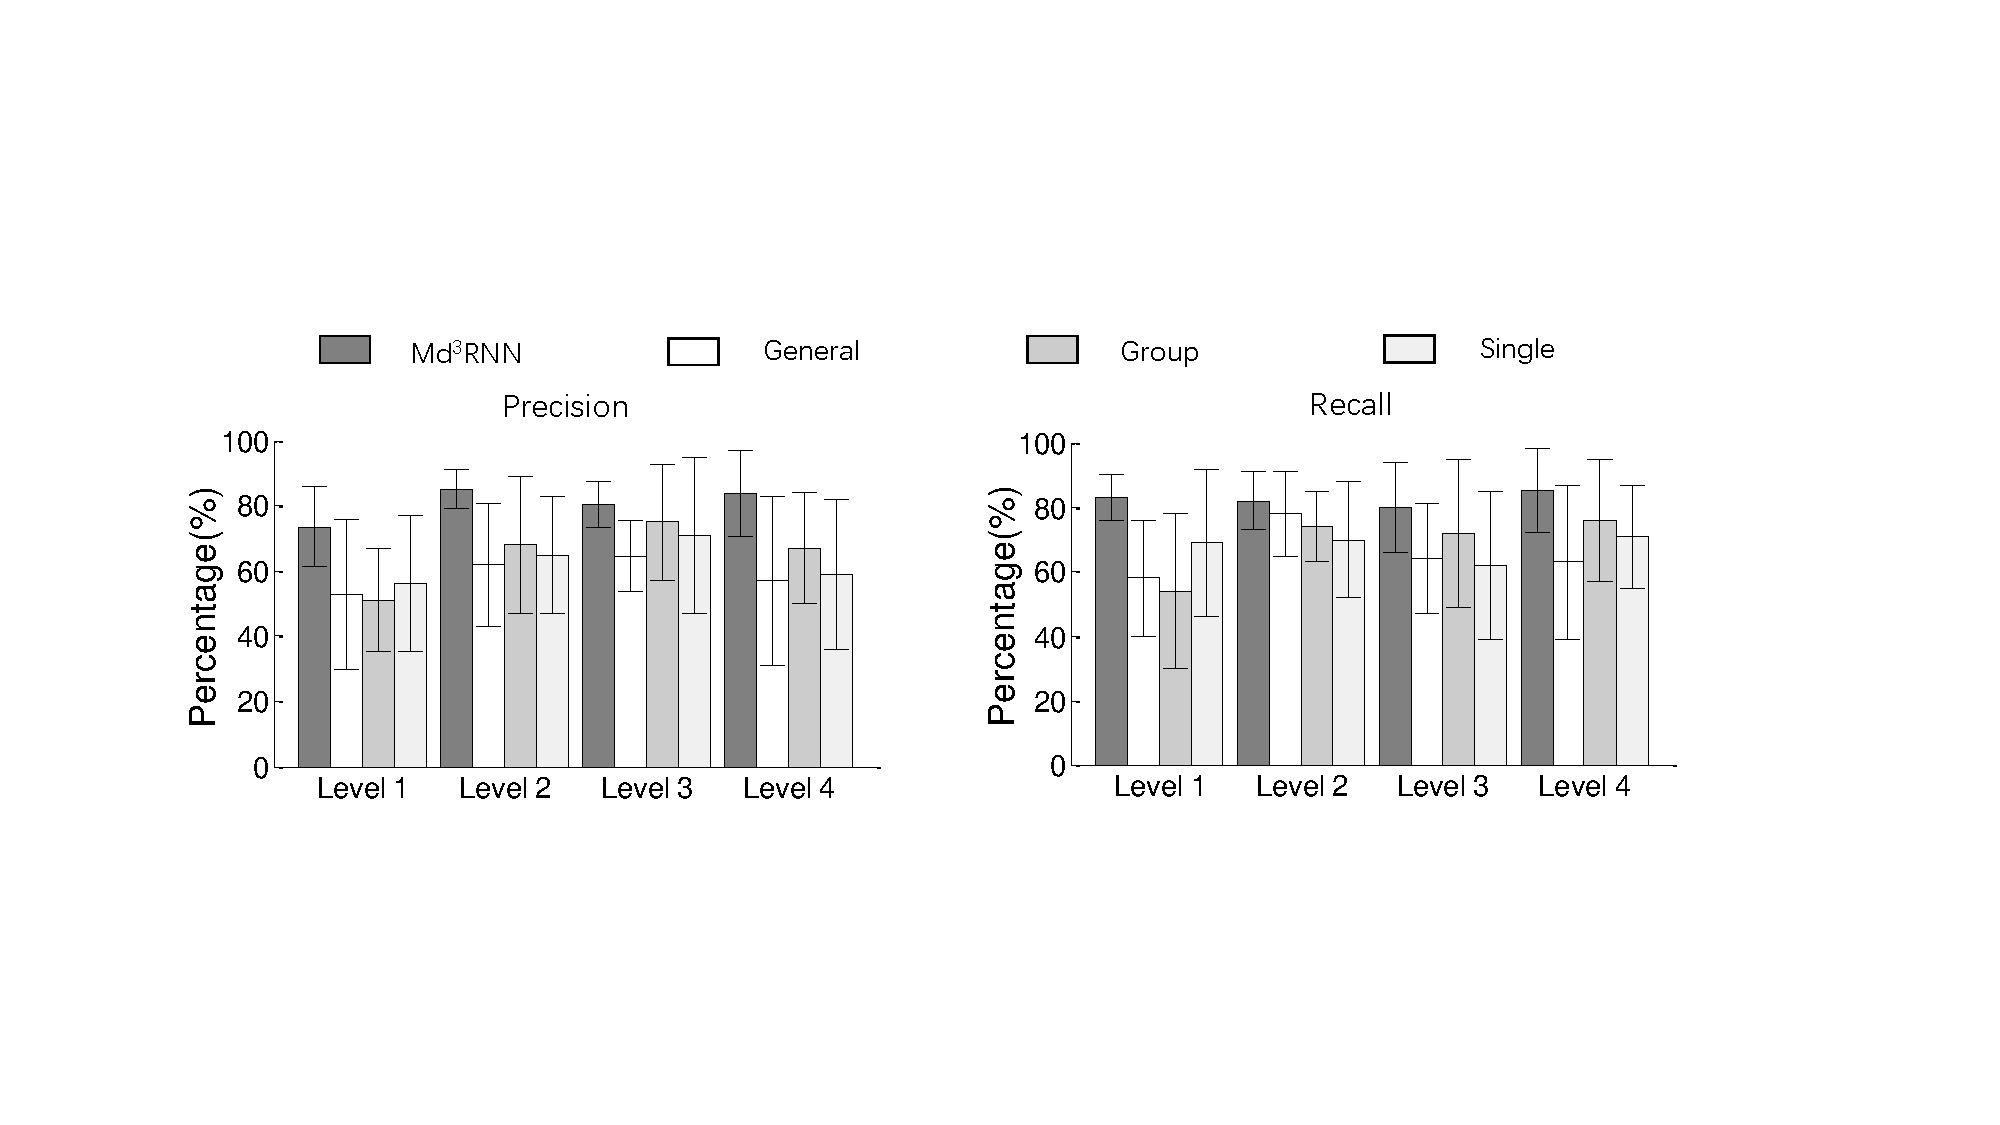
\includegraphics[width=0.8\columnwidth]{./img/performance_of_multi_division.pdf}
  \caption{Performance of data sharing schemes. \rev{The error bars denote the standard deviations on 10-fold cross-validation.}}
  \label{fig:cmp_multi_division}
\end{figure}


\subsubsection{Effectiveness of \modelname Learning Algorithm}
To demonstrate the effectiveness of adopting \modelname learning algorithms over other classifiers, we compare it with several typical algorithms from following  two aspects.

The typical classifiers that do not share features from users:  1) Support vector machine 2) Gaussian Process 3) Hidden Markov Model 4) Random Forest (RF) 5) Artificial neural network (ANN) 6) Gradient Boosting (GB).

\begin{itemize}
  \item
  \textbf{Random Forest (RF)~\cite{bib:liaw2002classification}.}
  As an ensemble method, RF combines many simple decision trees together and output the mode of classes for prediction.
  To avoid correlation among base trees, random set of features are selected in the splitting process when constructing each decision tree.

  \item
  \textbf{Artificial neural network (ANN)~\cite{bib:wang2003artificial}.}
  We also included the classical ANN as a baseline, simply to justify the benefit of ``structure engineering'' from \modelname. The ANN under comparison contains a single input layer, three hidden layers, and an output layer. The training of ANN is done by using the stochastic gradient descend algorithm implemented in Tensorflow \cite{bib:Tensorflow}.

  \item
  \textbf{Gradient Boosting (GB)~\cite{bib:friedman2002stochastic}.}
  GB generates a prediction model by combining many weak classifiers into a stronger classification committee.
  We use the implementation of the fastAdaboost \cite{bib:fastAdaboost} to combine basic tree classifiers for ensemble learning.

  \item
  \textbf{Support Vector Machines  (SVMs)~\cite{bib:wang2005support} .}
  Support vector machines (SVM)s are supervised learning models with efficient convex learning algorithms that are widely used for classification and regression analysis.
  The idea is to construct optimal separating hyperplane that maximizes the separation margin of two data groups (classes).
  Due to this geometric property, it usually generalizes well, and its dual form is a quadratic programming that can be easily incorporated with kernels, which allows an implicit transformation of the examples from the original space to a non-linear high dimensional Hilbert space for better separation. We adopt the implementation of SVM in \cite{bib:scikit-learn} for classification.

 \item
 \textbf{Gaussian Processes (GP)~\cite{bib:rasmussen2006gaussian}.}
  Instead of directly parameterizing a latent function for classification, GP~\cite{bib:rasmussen2006gaussian} models it with a generic Gaussian process, i.e., a distribution over the functional space of the classifier or regressor.
  The posterior of the process is updated with training data set, and is ``squashed'' through a logistic function for classification. The covariance matrix used in GP also allows the utilization of the "kernel trick" to capture similarities in some nonlinear space. The Gaussian process classifier utilized in this paper is provided by \cite{bib:scikit-learn}.

  \item
  \textbf{Hidden Markov model (HMM)~\cite{bib:rabiner1986introduction}.}
  A hidden Markov model (HMM) is a statistical Markov model in which the system being modeled is assumed to be a Markov process with unobserved (hidden) states. It can be presented as the simplest dynamic Bayesian network. Simple as it is, HMM has been widely used in signal processing and time series analysis due to its interpretability and tractability.

\end{itemize}

\rev{
The typical classifiers that share features from users. We use multiple task framework to share the information among users.
Each task indicates an user.
1) Multiple task Support Vector Machine (mSVM) 2) Multiple task Gaussian Processes (mGP) 3) Nested Dirichlet Process infinite Hidden Markov model (nDP-iHMM) 4) Multiple task Random Forest (RF) 5) Multiple task neural network (ANN) 6) Multiple task Gradient Boosting (GB).


\begin{itemize}
  \item
  \textbf{Support Vector Machine (mSVM) that allows information sharing.}

  We use a multiple task version of the SVM classifier proposed in~\cite{evgeniou2004regularized}, which incorporate the relation between tasks through a task-coupled kernel function.
  To eliminate scale/location discrepancies among input variables, all features are normalized before being used in the training phase.

  \item
  \textbf{Gaussian Processes (mGP) that allows information sharing.}
  The multi-task version of GP can be achieved by redefining the kernel matrix to include task similarities. We adopt the multi-task GP proposed in \cite{bonilla2007multi}, and also implement several approximation algorithms for acceleration \cite{bib:chalupka2013framework}.

  \item
  \textbf{Multiple Hidden Markov model that allows information sharing.}
  To further improve the model flexibility, the authors of \cite{ni2007multi} proposed the so-called Nested Dirichlet Process infinite Hidden Markov model (nDP-iHMM) based on a non-parametric method for possibly undetermined state space, and imposing a nested Dirichlet process prior to share information among tasks.
\end{itemize}

\figref{fig:cmp_models} illustrates the results.
Apparently, \modelname achieves best performance on both precisions and recalls.
More specifically, it outperforms the runner-up by at least 20\% in terms of average precision, and yields much better recalls for the categories of interest, \ie Level 1 and Level 4.
Among those baselines, it appears that no method could dominate the others, except that nDP-iHMM performs slightly better in terms of recall score.
This is mainly because nDP-iHMM is the only method among baselines that allows both temporal correlation and information sharing among tasks.
However, compared to \modelname, which is able to describe multi-scale dynamics, nDP-iHMM is still worse in general.
The dominating performance of \modelname is somewhat expected, as those baselines either ignore the multi-scale dynamics of the observed data, or can not allow information sharing among available data from users.
The above observation further justifies the efforts of designing the new machine learning paradigm for \sysname, which efficiently transfers valuable knowledge between individuals.
}

\begin{figure}[h]
  \centering
  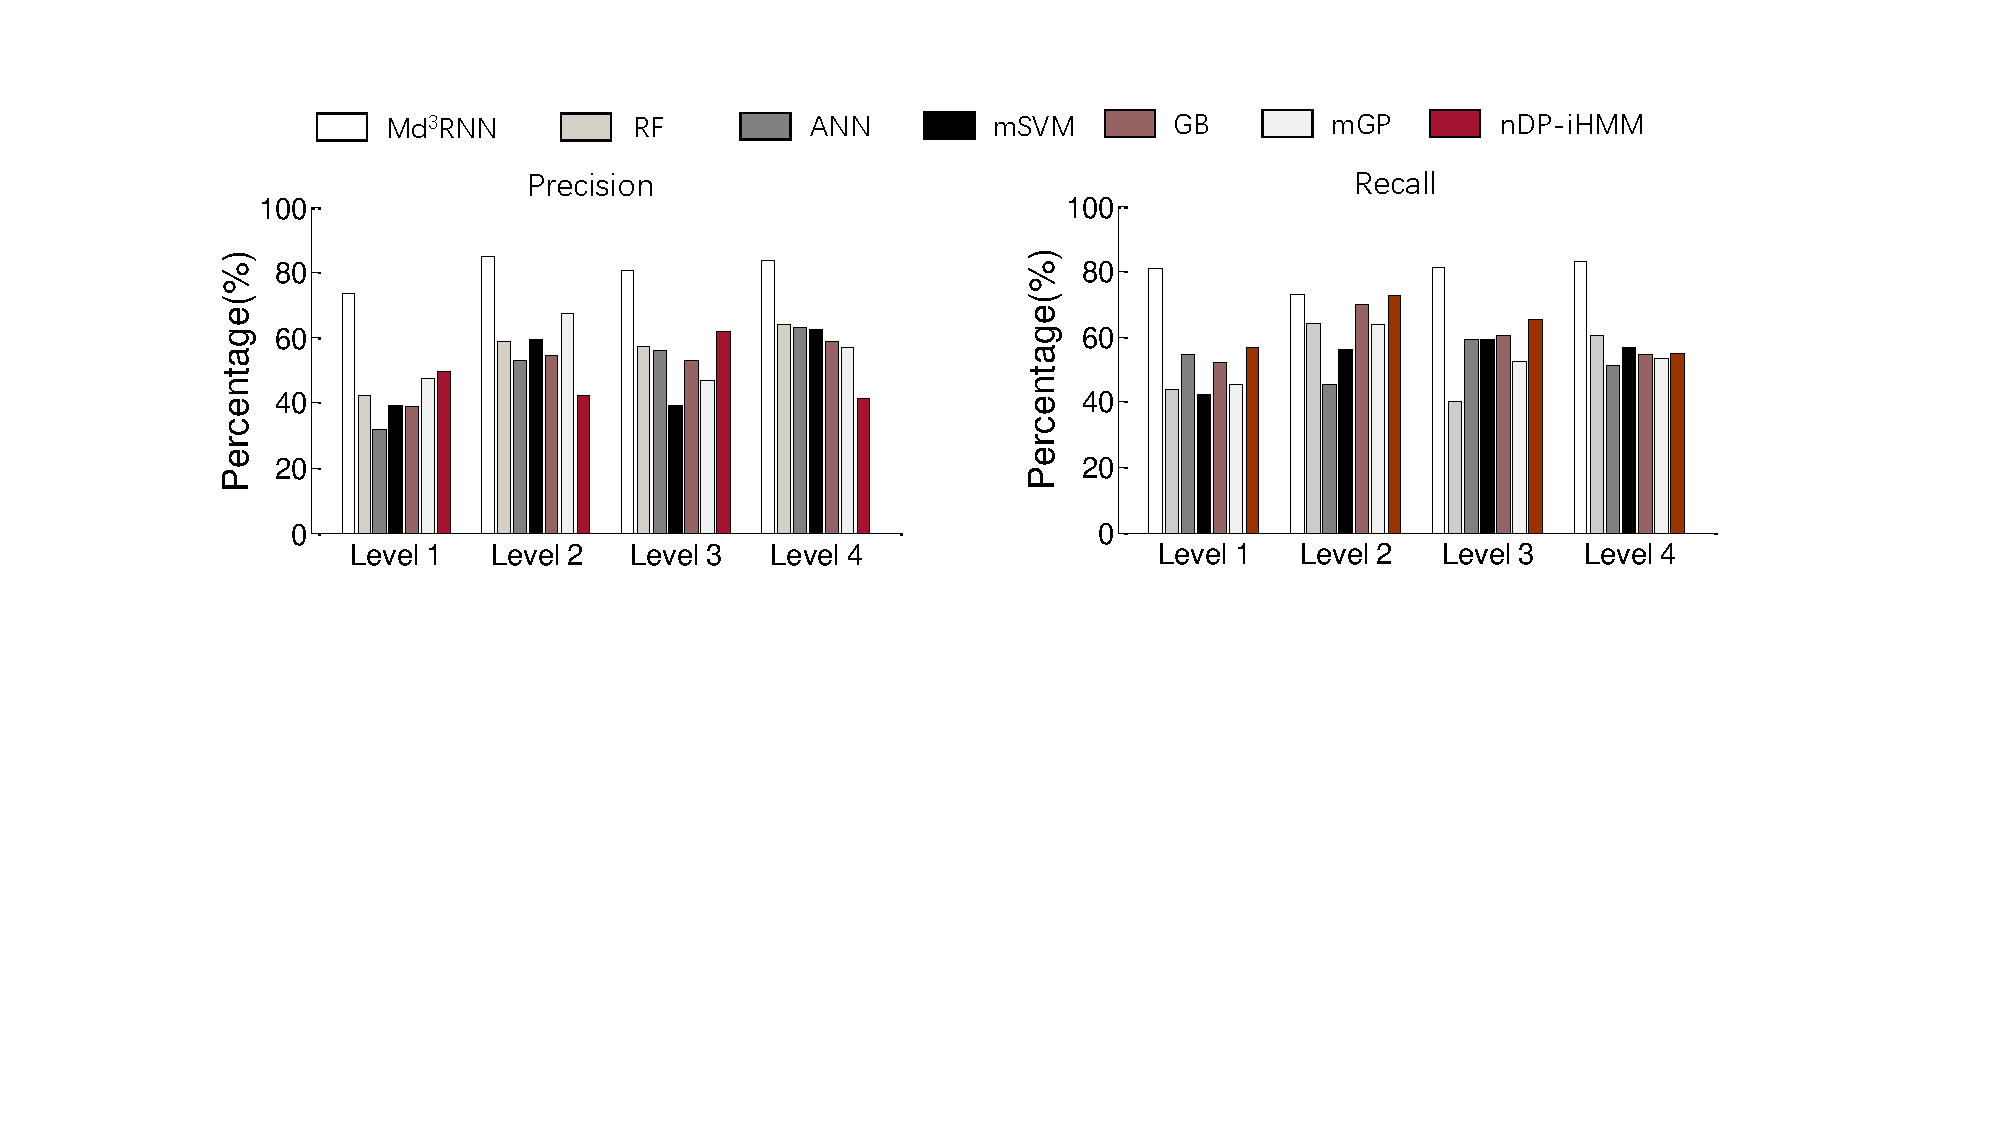
\includegraphics[width=0.8\columnwidth]{./img/Model_CMP1.pdf}
  \caption{Performance comparison with the different learning algorithms.}
  \label{fig:cmp_models}
\end{figure}

\subsection{Micro-benchmarks}
\subsubsection{Effectiveness of Features}
\tabref{tab:features} shows the average precisions and recalls using different combinations of features.
By combining physiological features ($X_{P}$) with temporal features ($X_{T}$), the average precision and recall of the 4 blood glucose levels improve by 31.38\% and 41.48\% respectively.
\rev{The precision and recall increase by about 10\% to 30\% with physiological and short-term temporal features ($X_{P}+X_{T_2}$) over physiological features alone.
However, the historical trends $X_{T_1}$ prove to be more effective than the short-term temporal features $X_{T_2}$ (see the second and the third rows of \tabref{tab:features}).
The necessity to include historical trends indicates the need for re-calibration, as will be discussed in \secref{subsubsec:gaps}.
}

\begin{table}[h]
  \small
  \centering
  \caption{Effectiveness of features.}
  \label{tab:features}
  \begin{tabular}{|c|c|c|c|c|c|c|c|c|}
  \hline
  & \multicolumn{2}{c|}{\textbf{Level 1}} & \multicolumn{2}{c|}{\textbf{Level 2}} & \multicolumn{2}{c|}{\textbf{Level 3}} & \multicolumn{2}{c|}{\textbf{Level 4}}                     \\ \hline
  \textbf{Features} & \textbf{Precision} & \textbf{Recall} & \textbf{Precision} & \textbf{Recall} & \textbf{Precision} & \textbf{Recall} & \textbf{Precision} &\textbf{Recall}
  \\ \hline
  $X_{P}$ & 43.37$\%$ & 32.82$\%$ & 46.03$\%$ & 39.10$\%$ & 51.79$\%$ & 48.95$\%$ & 56.30$\%$ & 43.49$\%$
  \\ \hline
  $X_{P}$+$X_{T_1}$ & 58.29$\%$ & 63.60$\%$ & 72.15$\%$ & 60.17$\%$ & 68.84$\%$ & 61.49$\%$ & 73.23$\%$ & 66.74$\%$
  \\ \hline
  \rev{$X_{P}$+$X_{T_2}$} & \rev{54.48$\%$} & \rev{49.11$\%$} & \rev{50.81$\%$} & \rev{69.43$\%$} & \rev{67.21$\%$} & \rev{70.20$\%$} & \rev{61.24$\%$} & \rev{64.10$\%$}
  \\ \hline
  $X_{P}$+$X_{T_1}$+$X_{T_2}$ & 73.62$\%$ & 83.13$\%$ & 85.12$\%$ & 81.96$\%$ & 80.55$\%$ & 79.97$\%$ & 83.72$\%$ & 85.23$\%$
  \\ \hline
  \end{tabular}
\end{table}


\subsubsection{Necessary Training Data}
In this experiment, we evaluate the performance of \sysname with increasing numbers of training samples.
Since the duration of measurements for each participant varies from 6 to 30 days, we use measurements of 5 to 25 days for training, and the rest for testing.
Note that we keep the measurements for training but exclude them for testing if the duration of certain user's measurements is insufficient.
For example, if the user's measurements last for 7 days, we use his measurement to evaluate the performance of using 5 days of training data, and test on the measurements of the remaining 2 days.
However, when evaluating the performance with 10 days of training data, we only use his 7 days of measurements for training, but not for testing.

\begin{figure}[h]
  \centering
  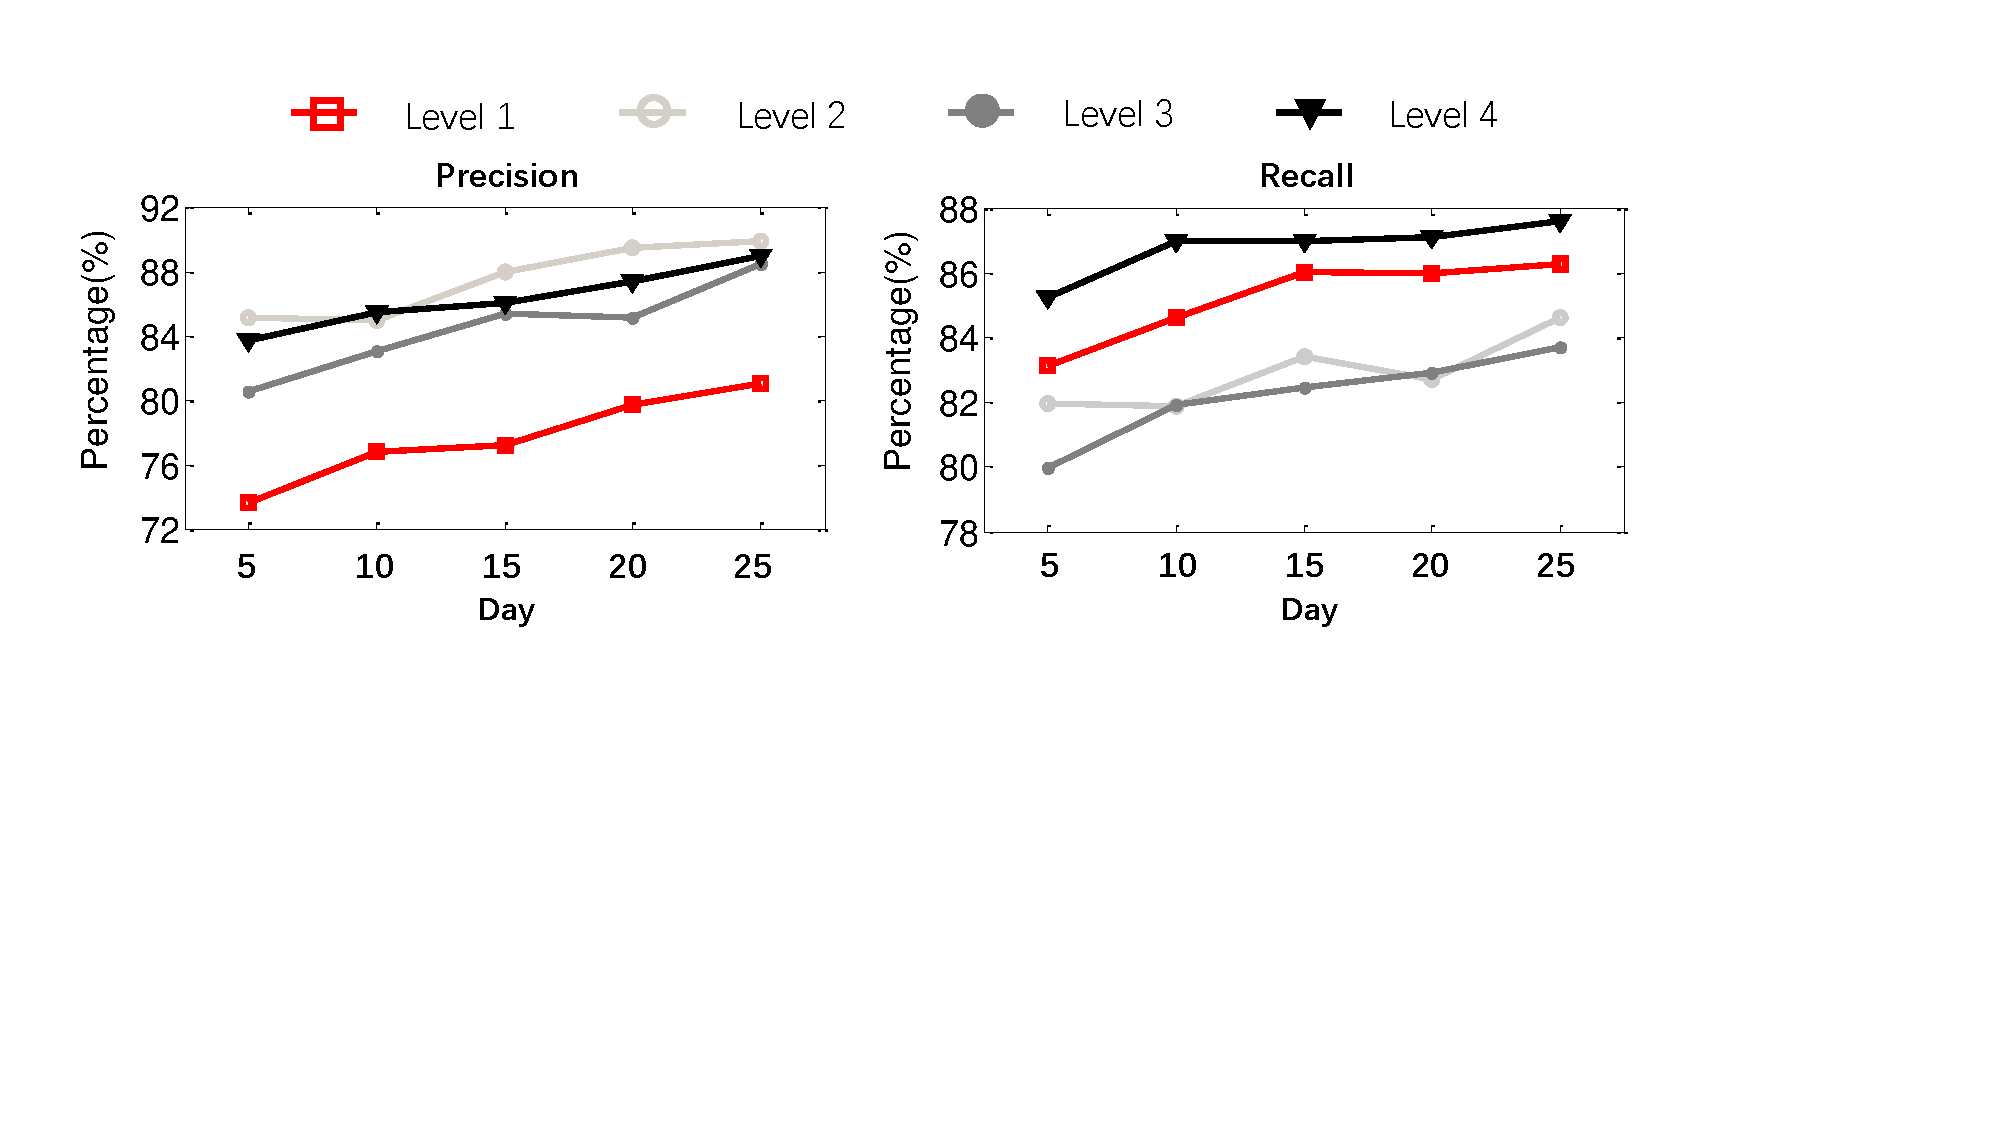
\includegraphics[width=0.8\columnwidth]{./img/performance_under_days1.pdf}
  \caption{Impact of increasing amount of training samples.}
  \label{fig:per_under_train_days}
\end{figure}

\figref{fig:per_under_train_days} illustrates the results for all the 4 blood glucose levels.
The results are averaged over all testing samples as in previous evaluations.
As expected, the precisions and recalls for all the 4 blood glucose levels improve smoothly with the increase of training samples.
The results verify that the challenge (and our motivation to adopt a multi-division deep learning framework) is the lack of training data.
Note that \sysname is not a replacement of the current CGM devices, but rather, a complement when CGM devices are uncomfortable or inconvenient to wear.
Therefore we envision the training dataset will grow gradually after wearing the CGM device multiple times (at least for diabetes patients), and the overall accuracy will also improve over time as a result.



\subsubsection{Impact of Temporal Gaps}
\label{subsubsec:gaps}

The blood glucose concentration is correlated with the previous blood glucose levels because of the control loop of the glucose metabolism~\cite{bib:TBE07:Dalla, bib:PE04:Hovorka, bib:IJNMBE16:Oviedo}.
Since \sysname does not rely on the previous blood glucose value measured by CGM as an input, it is natural that the accuracy of \sysname will degrade if there is a long gap between the training and the testing datasets (\ie the training dataset can be outdated).
\rev{To demonstrate this point, we adopt the first 5 days of measurements as training set, and increase the testing measurement gap  by 5 days gradually.}

\begin{figure}[h]
  \centering
  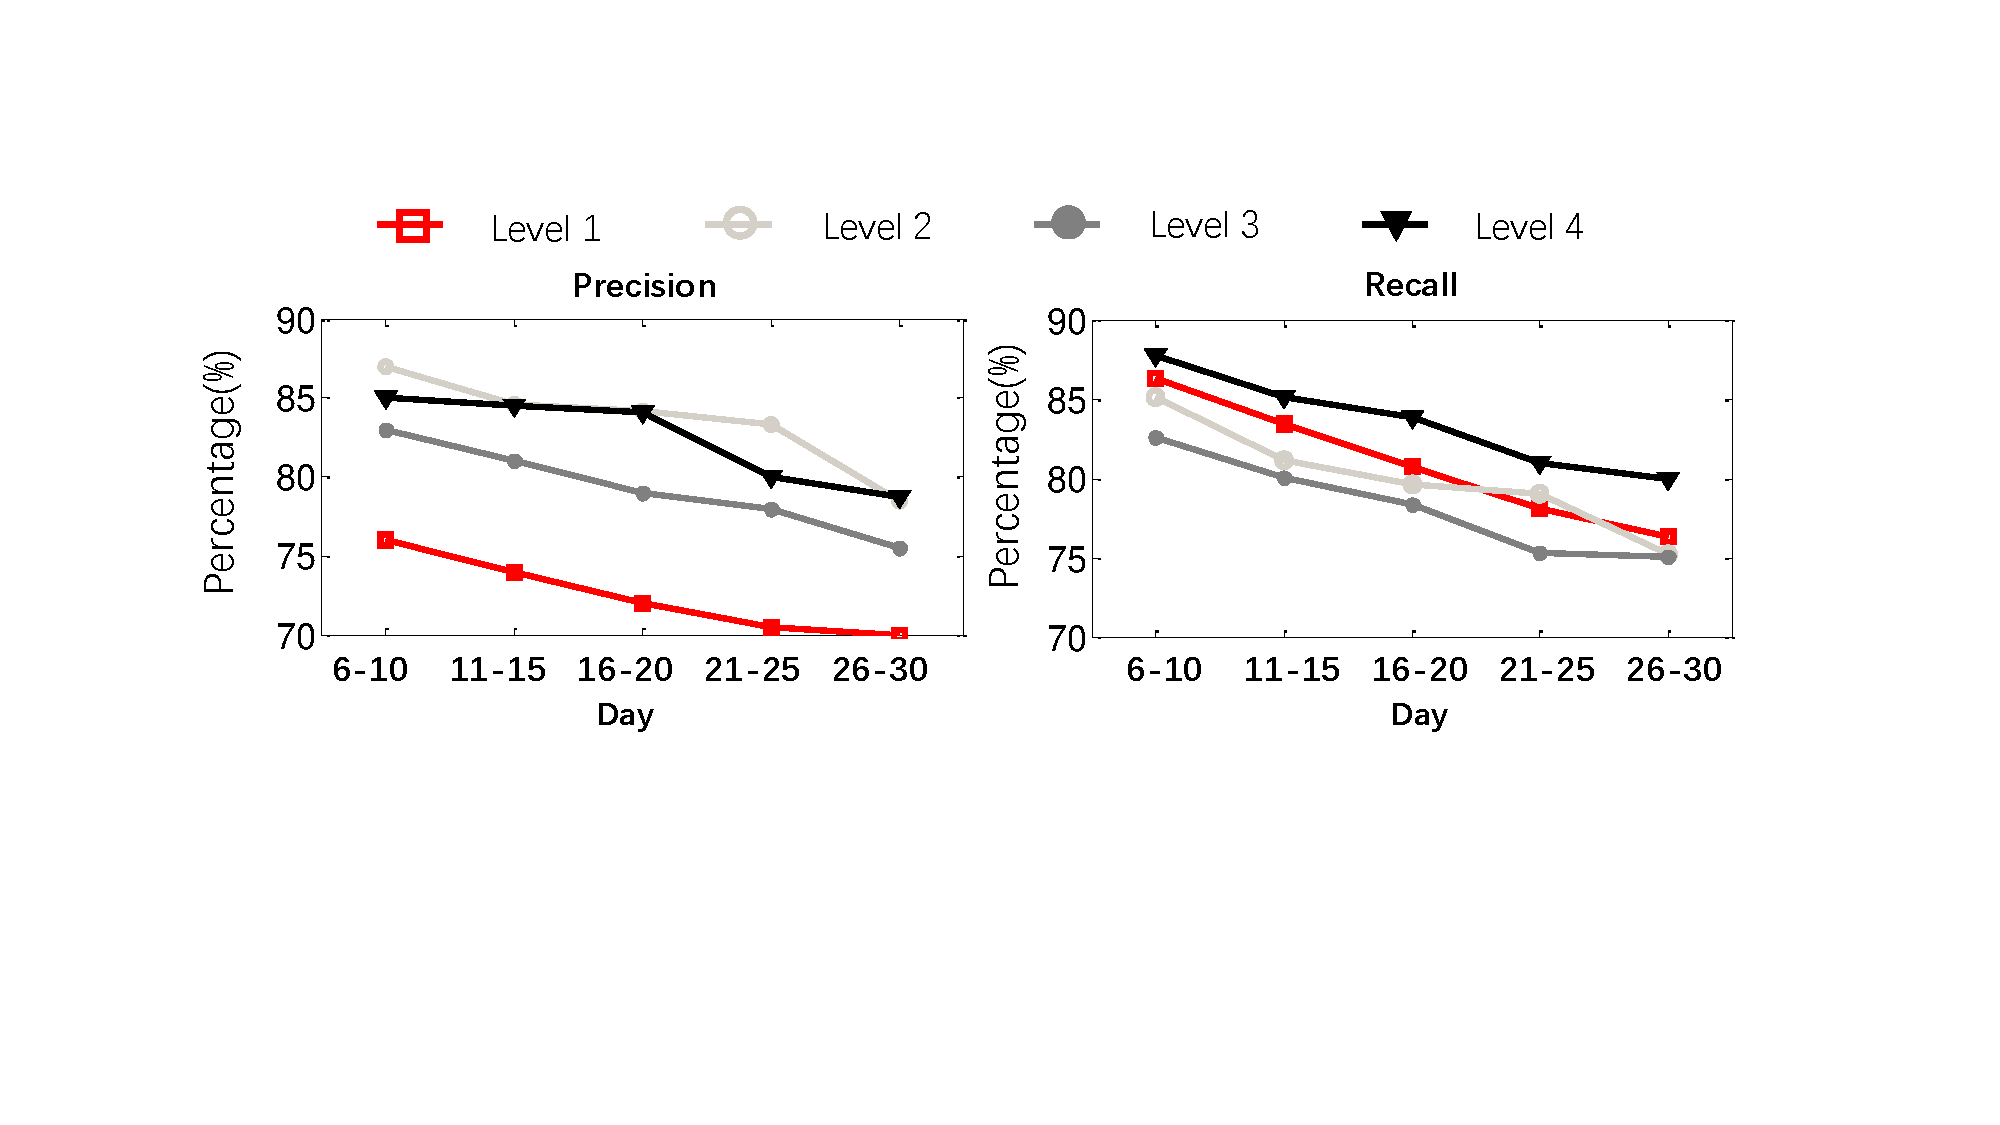
\includegraphics[width=0.8\columnwidth]{./img/Performance_gap2.pdf}
  \caption{Impact of temporal gaps between the training and testing datasets.}
  \label{fig:per_under_various_pred_days}
\end{figure}

\figref{fig:per_under_various_pred_days} plots the overall performance of training using the same 5 days of measurements, and testing on measurements collected on the 6-10th, 11-15th, 16-20th, 21-25th, and 26-30th days, respectively.
As expected, both the precisions and recalls drop moderately with the increase of temporal gaps between the training and the testing datasets, with a maximum decrease of 6.73\% and 7.02\% in average precision and recall after 21-25 days.
\rev{Note that \sysname is not designed as a replacement of the commercial CGM devices, but rather an ubiquitous temporary alternative when CGM devices are uncomfortable or inconvenient to wear.
From the results, we suggest users to have a double-check while they receive a warning by \sysname, and recommend users to put on the CGM device to monitor the blood glucose at least every three weeks. For practice usage, users can observe their blood glucose dynamics by \sysname in business days, and wear CGM at leisure time \eg weekends or holidays.
The data sampled by the CGM will automatically feed into \sysname for a model retraining, guaranteeing the inference performance.
The current system, therefore, requires training from a CGM (like many previous works) and also requires periodic retraining to remain effective.}

\rev{
\subsubsection{Energy overhead}
\begin{table}[t]
  \centering
  \caption{Profiles of smartphone }
  \label{tab:smartphone_profiles}
  \begin{tabular}{|l|l|l|l|l|l|}
  \hline
  \textbf{Type} & \textbf{CPU}    & \textbf{RAM} & \textbf{ROM} & \textbf{Power Capacity} & \textbf{Operation System} \\ \hline
  Galaxy S6     & 8-cores 2.1 GHz & 3 GB         & 32 GB        & 2550m Ah                & Android 5.0               \\ \hline
  HTC Desire A6 & 8-cores 1.7 GHz & 2 GB         & 16 GB        & 2600m Ah                & Android 5.0               \\ \hline
  HUAWEI 4C     & 8-cores 1.2 GHz & 2 GB         & 8 GB         & 3100m Ah                & Android 4.4               \\ \hline
  LenovoK80M    & 4-cores 1.8 GHz & 4 GB         & 64 GB        & 4000m Ah                & Android 4.4               \\ \hline
\end{tabular}
\end{table}

Let us recall the system workflow from the energy overhead perspective.
\sysname triggers the microphone, the accelerometer and the light sensor after the user choosing the sleeping mode, which is utilized to track the sleep quality of users.
After the user waking up, \sysname shuts down the microphone and light sensor, only leaving an accelerometer to record the user's activities.
Thus, \sysname conserves energy from two aspects: first, it keeps the sensors activated only around the right time; second, it adopts low-power sensors to reduce energy consumption.

To evaluate the battery conditions, \sysname are tested on four popular types of commercial phones (listed in \tabref{tab:smartphone_profiles}) by volunteers.
All of the smartphones are charged full of power (100\% percentage).
Since \sysname is a service that could run in backstage, we lock the screen during this process and shut down all the applications except \sysname and a battery tracing application \cite{bib:PowerTutor}, which is installed in each smartphone to record the rest battery storage every two hours.
\figref{fig:battery_lifetime} illustrates the phone��s left battery as a function of execution time of \sysname.

\begin{figure*}[h]
  \centering
  \begin{minipage}{0.35\columnwidth}
  \centering
  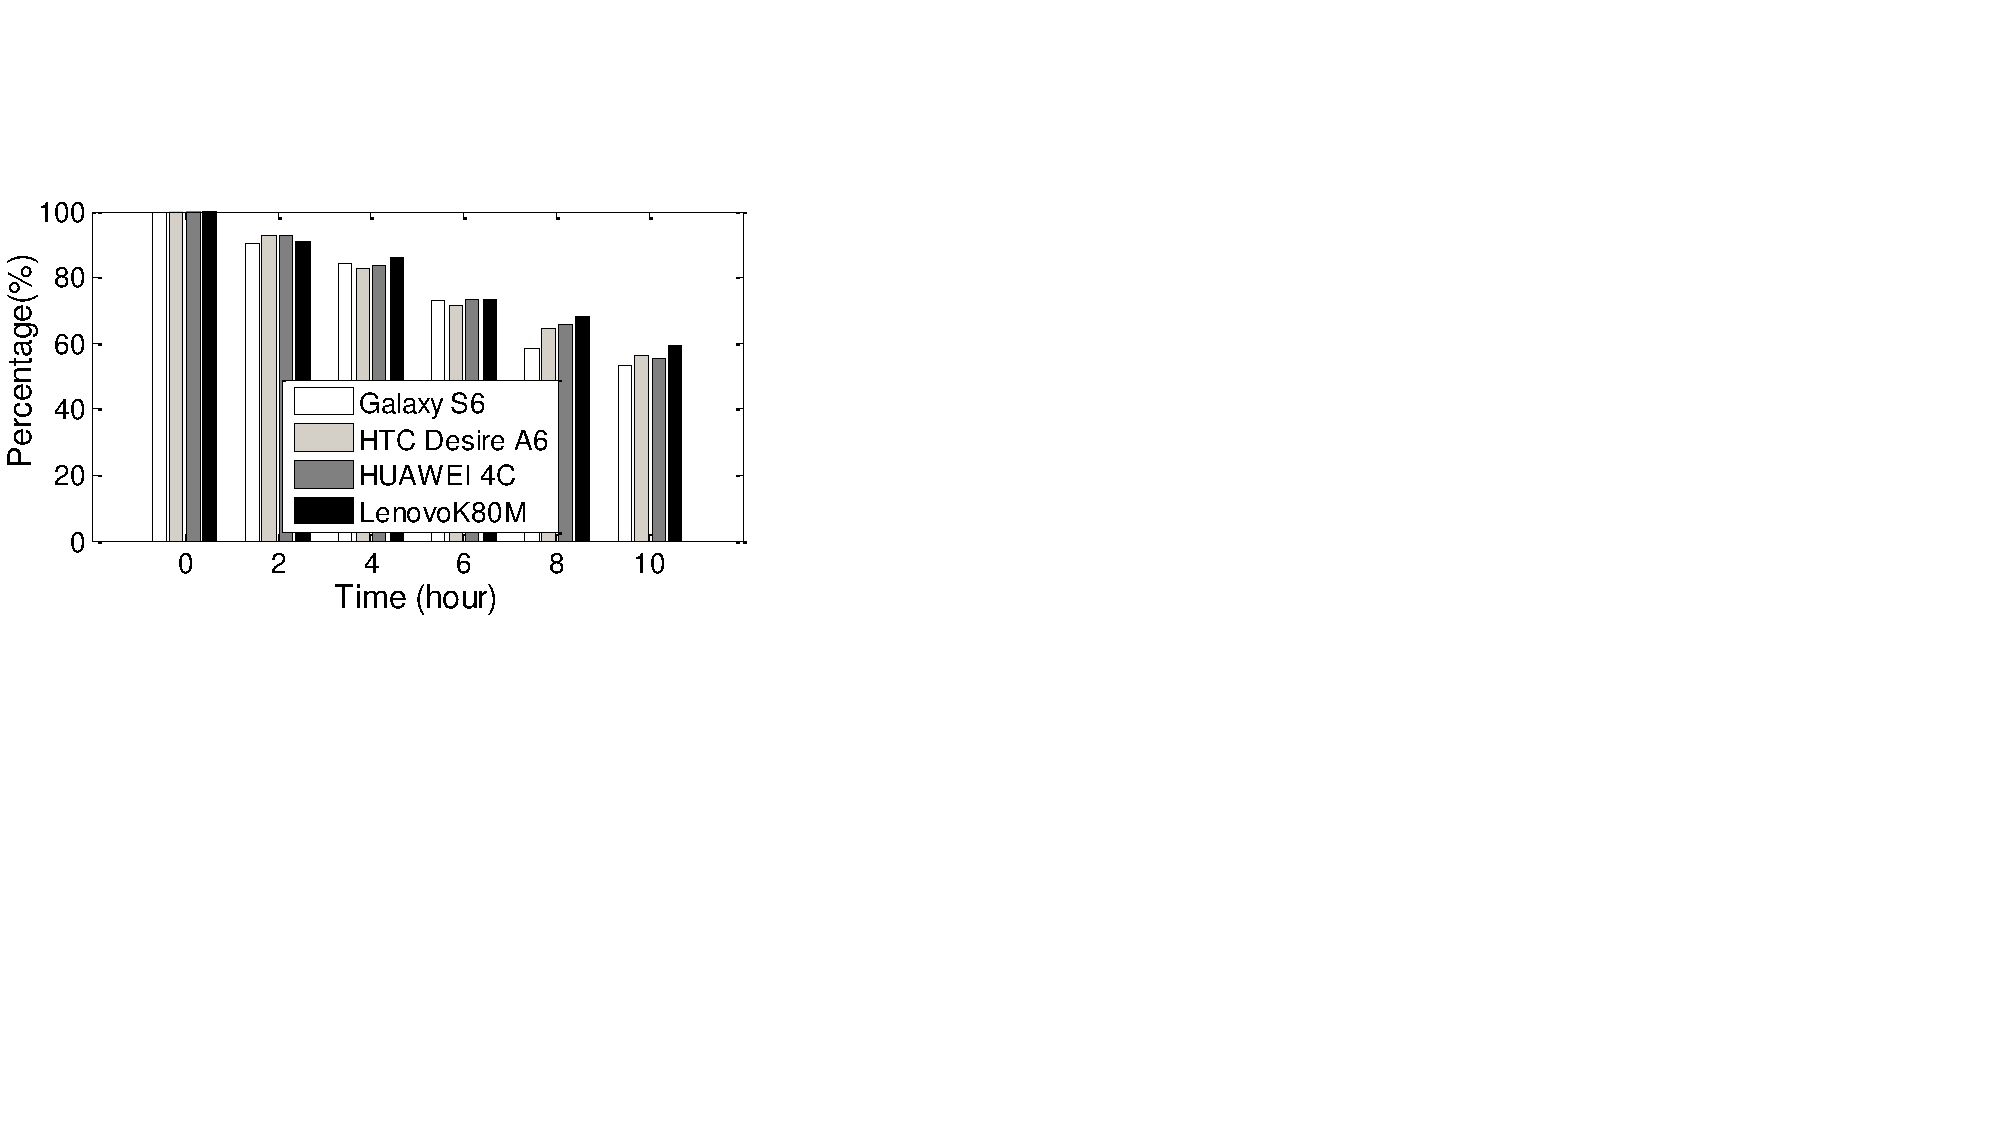
\includegraphics[width=1\columnwidth]{./img/battery_trace.pdf}
  \caption{Battery lifetime trace}
  \label{fig:battery_lifetime}
  \end{minipage}
  \hspace{0.05\columnwidth}
  \begin{minipage}{0.5\columnwidth}
  \centering
  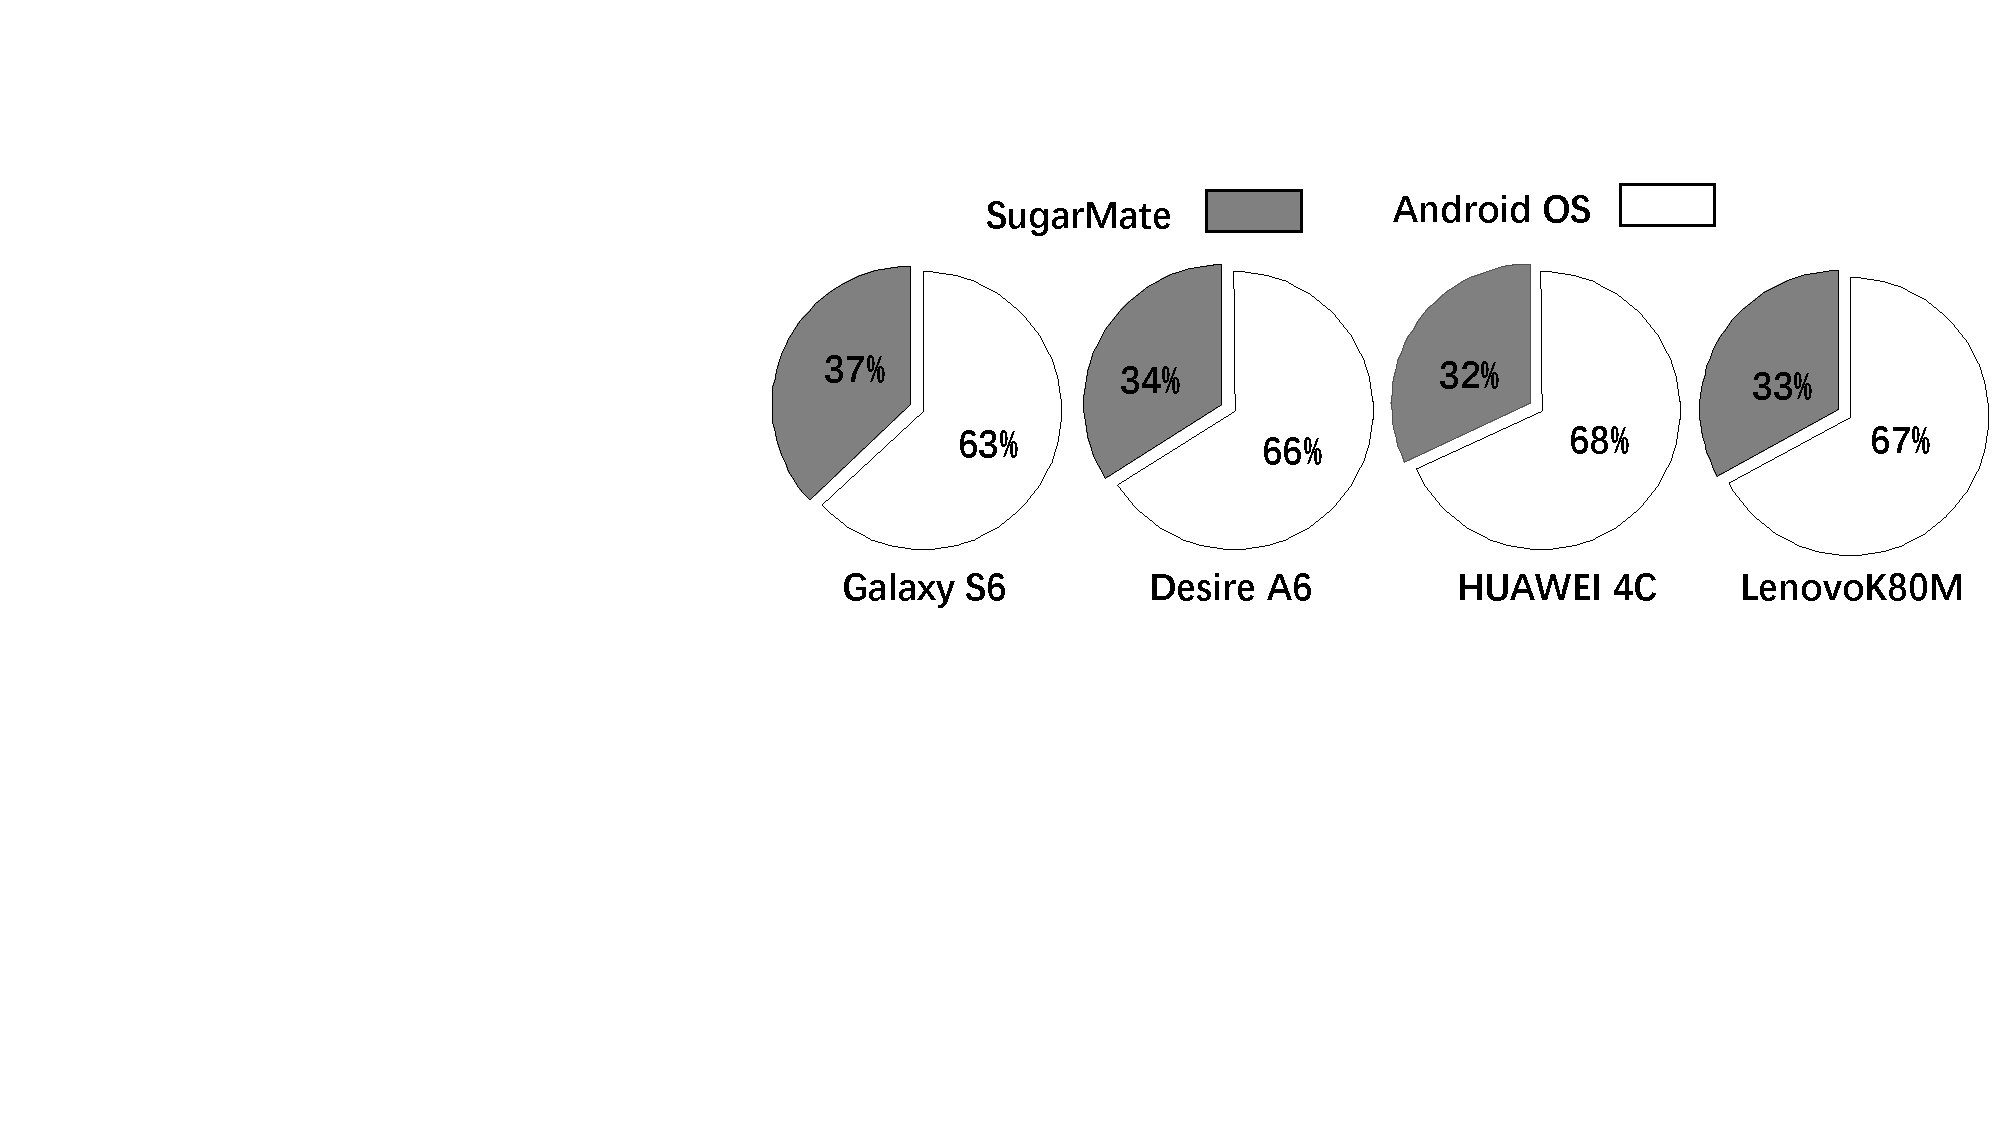
\includegraphics[width=1\columnwidth]{./img/energy_overhead.pdf}
  \caption{Battery consumption distribution}
  \label{fig:battery_consumption}
  \end{minipage}%
\end{figure*}

As it indicates, the energy consumption presents a similar trend yet differs in amount for all of these four phones.
Specifically, \sysname consumes energy around 10\% on average every two hours. With time passing by, the cumulative energy consumption increases
gradually, and finally ends up with about 50\% $\sim$ 60\%.

\figref{fig:battery_consumption} details the distribution of battery consumption in the experiments.
\sysname only consumes less than 40\% of the whole energy, most power is costed by Android OS.
That is to say, \sysname only costs less than 4\% battery every two hours, which is negligible and
affords for the daily use.

}
